% \section{Center Embedding Leads to The Hierarchical Rule}
\section{Data Complexity Determines Rule Preference}
\label{sec:data_complexity}

We find that models generalize hierarchically because they are trained on data which includes center embeddings, a linguistic structure which we describe in Section \ref{sec:center_embed}. Center-embedded sentences drive hierarchical generalization in both the QF task (Section \ref{sec:qf_result}) and the TI task (Section \ref{sec:ti_result}).

\begin{figure}[t!]
    \centering
    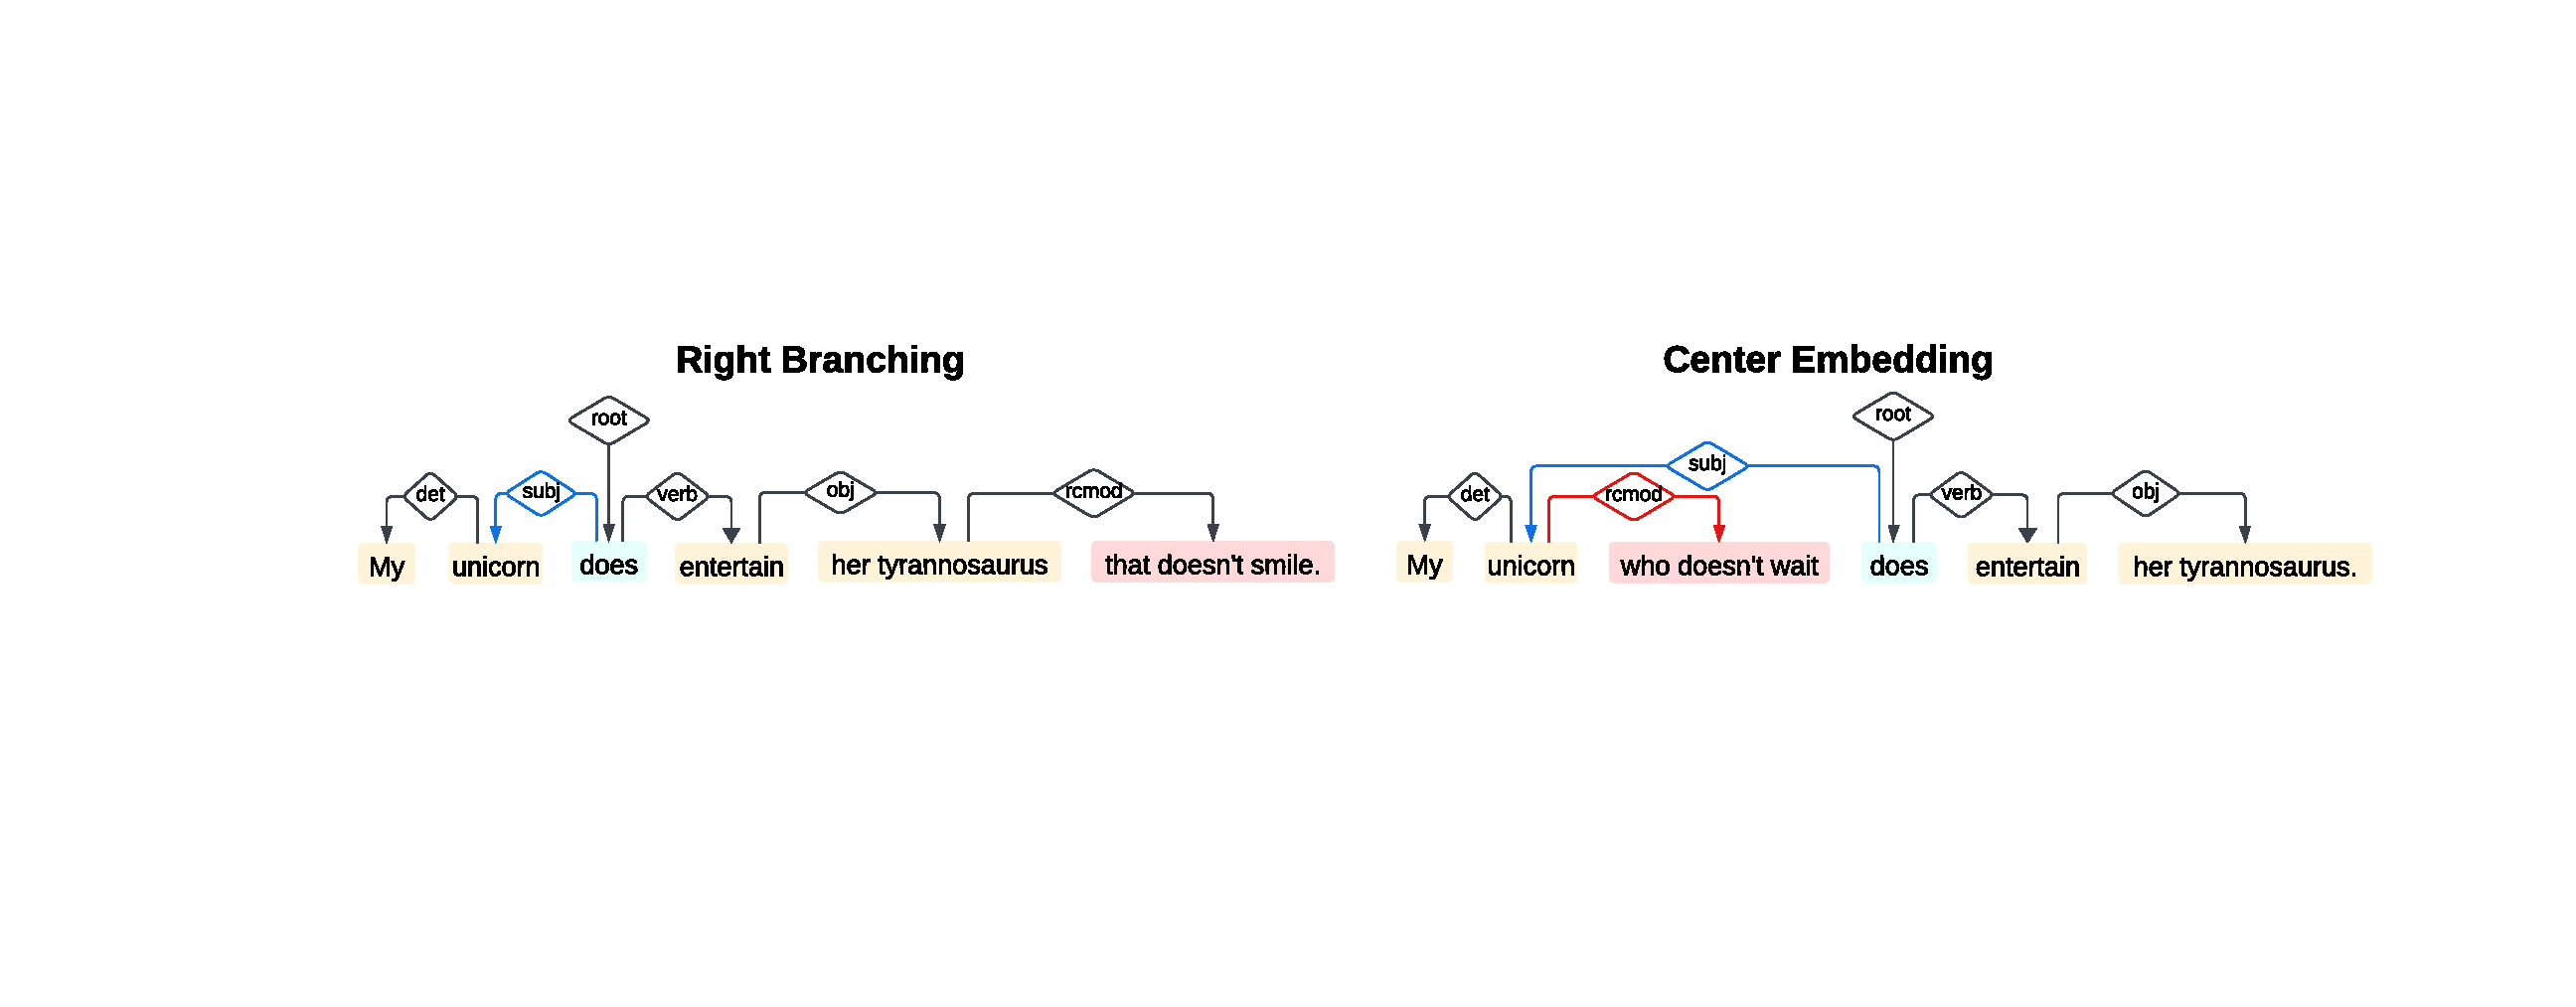
\includegraphics[width=1.0\textwidth]{figures/sentence_demo.pdf}
    \caption{\textbf{Sentence Examples.}   \textit{Left:} Right-branching sentence example. The linear progression of the main constituent is not interrupted by the relative clause. 
    \textit{Right:} Center-embedded sentence example. When the relative clause modifies the subject, it interrupts the linear progression of the main constituent. 
    }
    \label{fig:sentence_demo}
\end{figure}

\subsection{Center Embedding}
\label{sec:center_embed}
Center embedding occurs when a clause is placed recursively within another clause of the same type. Figure \ref{fig:sentence_demo} (\textit{left}) illustrates two examples of center-embedded sentences, where the embedded clause complicates syntactic parsing by placing an additional subject noun in between a verb and its own subject. Whereas center embeddings exhibit a recursive structure, sentences without center embeddings are exclusively right-branching. Right-branching structures may also include modifying clauses, but these clauses can only be appended at the end of the main clause, maintaining its linear flow (see Figure \ref{fig:sentence_demo}, \textit{right}). Linguists have long argued that center embeddings play a crucial role in grammar acquisition \citep{wexler1980formal} and give rise to tree-like syntactic structures \citep{Chomsky2015-bg}. 


We find that center embeddings, which are crucial for human language acquisition, also lead an LM to acquire hierarchical grammar rules. To correctly predict the next token, LMs must track syntactic connections between words in the context. In right-branching sentences, LMs can rely on linear proximity to identify these connections; as shown in Figure \ref{fig:sentence_demo}, a simple bigram model suffices to capture the subject-verb relationship for such sentences. In contrast, center embeddings introduce relative clauses of various lengths, making linear n-gram models inefficient for capturing subject-verb relationships. The recursive nature of the center embedding requires the model to track multiple subject-verb relationships: one for the main clause and a separate one for the embedded relative clause. In these cases, a tree structure is more efficient to model subject-verb relationships. 


\subsection{Question Formation Results}
\label{sec:qf_result}
As specified in Section \ref{sec:qf_task}, the training data for QF is ambiguous between the linear rule (i.e., moving the first auxiliary) and the hierarchical rule (i.e., moving the main auxiliary). Center-embedded sentences do not meet this ambiguity requirement and, therefore, cannot appear in question formation training samples. To ensure the model is exposed to diverse sentence types, \citet{McCoy2018-uv} introduced a secondary task to the QF training dataset: declaration copying. Like question formation, the declaration-copying example starts with a declarative sentence, but instead of transforming it, the model simply repeats it. Since the ambiguity requirement only applies to the primary question formation task, declaration-copying examples can include center embeddings. Concrete examples of both tasks can be found in Appendix \ref{appdx:data_sample}.


We train models on three modifications of the original training data, varying the composition of the declaration-copying subset. 
In \textit{Quest Only}, we remove all declaration-copying examples.
In \textit{Center embed}, we only keep center-embedded examples. In \textit{Right branch}, we only keep right-branching examples. 
Every modified training sets retains all examples of the primary task, question formation.
Every model trained, regardless of its training set composition, reaches 100\% in-distribution validation accuracy; however, the OOD generalization performance, shown in Figure \ref{fig:grokking_selection} (\textit{left}), differs significantly across the modified training sets. 

Our results confirm that declaration copying examples, specifically center embeddings, are essential for inducing hierarchical generalization.
Models trained without any declaration-copying examples fail to achieve an OOD accuracy above 75\%; so do models trained \textit{only} on right-branching  declaration-copying examples. When trained instead \textit{only} on center-embedded declaration-copying examples, models exhibit a strong preference for the hierarchical rule. This evidence suggests that center-embedded sentences direct a model towards the hierarchical rule. 

\begin{figure}[t!]
    \centering
    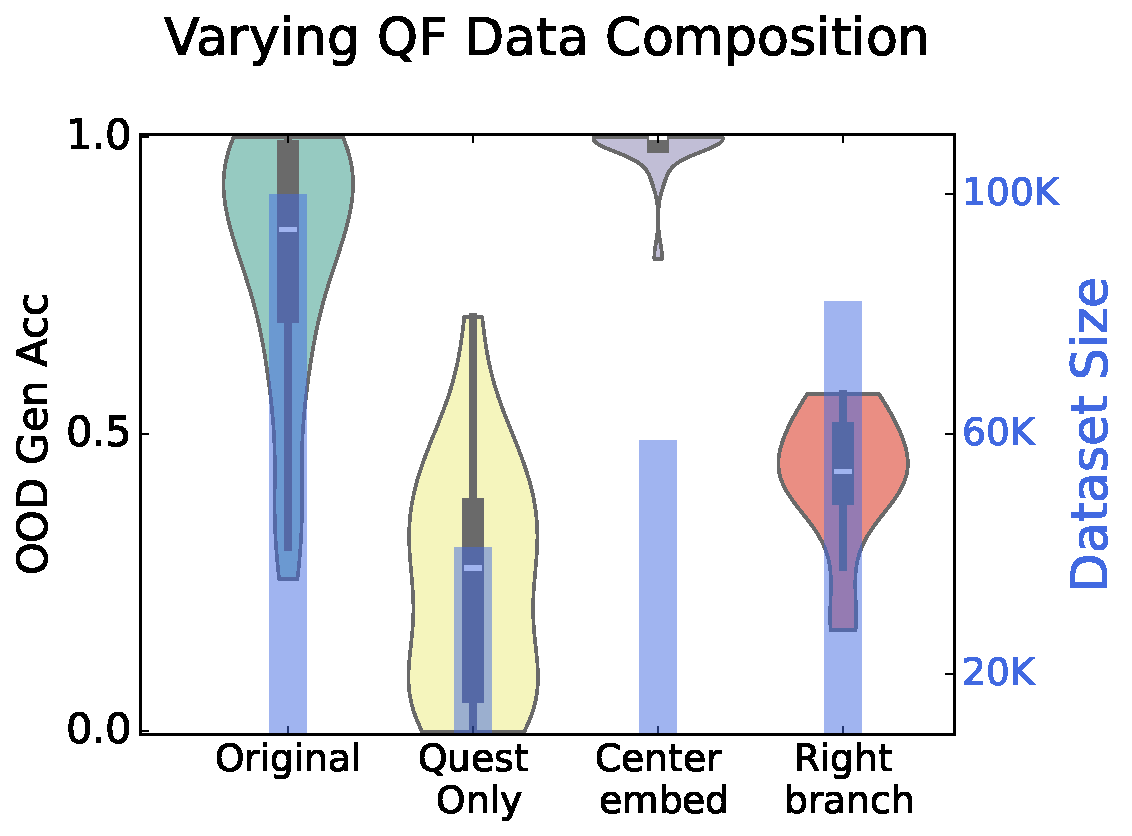
\includegraphics[width=0.41\linewidth]{figures/no_curriculum_main.pdf}
    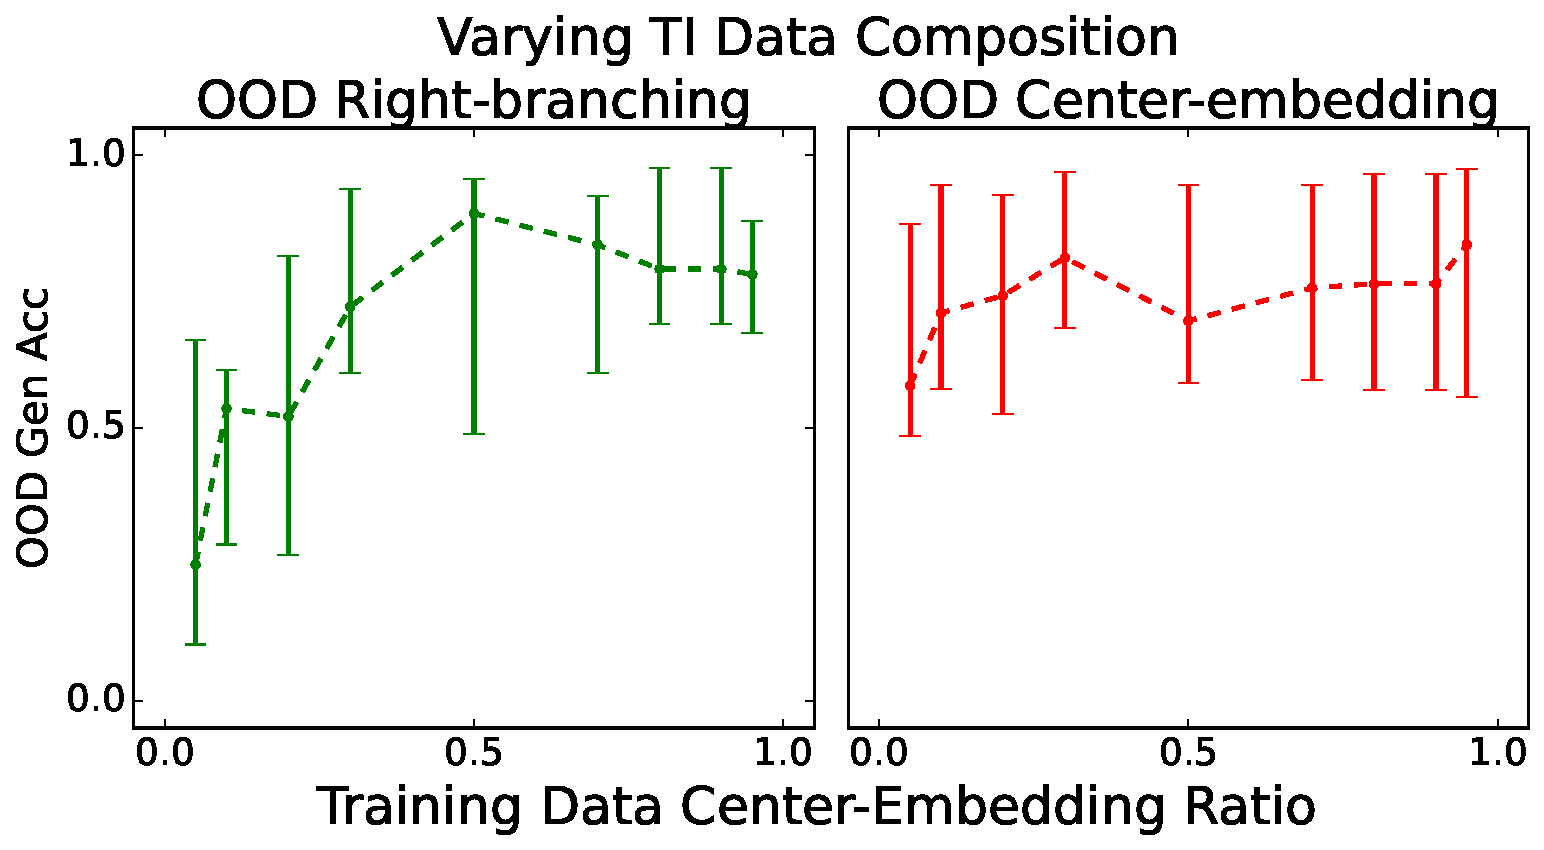
\includegraphics[width=0.55\linewidth]{figures/ti_simplicity_contamination.pdf}
    \caption{
    \textbf{Components of training data drive different generalization behaviors.} 
    \textit{Left:} Center-embedded sentences, which in the QF training data only appear in declaration copying examples, induce hierarchical generalization.
    \textit{Right:} Models are trained on different TI training data mixes and evaluated on two OOD sets: unambiguous right-branching sentences (\textit{green}) and unambiguous center-embedded sentences (\textit{red}). For center-embedded sentences, the hierarchical rule is preferred regardless of data mixes. For right-branching sentences, the model's preference for the hierarchical rule is exclusively driven by having a large mix of center-embedded sentences in the TI training data.}
    \label{fig:grokking_selection}
\end{figure}



\subsection{Tense Inflection Results}
\label{sec:ti_result}

In the TI training data, both right-branching and center-embedded sentences are made ambiguous by ensuring the distractor noun (i.e., a noun that appears between the main subject and the main verb) shares the same plurality as the main subject. For right-branching sentences, the distractor noun occurs in a prepositional phrase. For center-embedded sentences, the distractor noun occurs in a relative clause; either the subject or the object of the modifying clause can act as the distractor noun. We list examples below: 

\begin{enumerate}[itemsep=2pt,labelindent=10pt,topsep=0pt,parsep=0pt,partopsep=1pt, align=left, leftmargin=*]
    \item \textbf{Right Branching}: The noun in the prepositional phrase (e.g., `` \textit{to the cabinet}") acts as the distractor in the TI task.
    
    Example A (ID): \textit{The keys to the \textbf{cabinets} are on the table.}

    Example B (OOD): \textit{The keys to the \textbf{cabinet} are on the table.}
    
    \item \textbf{Center Embedding}: Either the subject or the object inside the relative clause acts as the distractor in the TI task.

    Example C (ID): \textit{The keys that unlock the \textbf{cabinets} are on the table.}

    Example D (OOD): \textit{The keys that unlock the \textbf{cabinet} are on the table.}
    
    
\end{enumerate}
We create variations of the TI training data by adjusting the ratio of right-branching to center-embedded samples while keeping the total training size constant.\footnote{The original training dataset contains a secondary past-tense copying task, to parallel the declaration-copying secondary task in QF. We show in Appendix \ref{appdx:ti_secondary} that the secondary task is not necessary, and we do not include it in our modified training sets.} A model's generalization behavior is tested on two OOD sets: one containing unambiguous right-branching sentences (e.g., Example B) and the other containing unambiguous center-embedded sentences (e.g., Example D). 

Generalization accuracies are shown in Figure \ref{fig:grokking_selection} (\textit{right}). When the training data is dominated by ambiguous right-branching sentences, the model fails to learn the hierarchical rule, as indicated by low OOD accuracy. However, when trained on a greater proportion of center-embedded sentences, the model systematically applies the hierarchical rule to both right-branching and center-embedded OOD sentences. As shown in Figure \ref{fig:grokking_selection} (\textit{right}), regardless of its training data mix, the model  generalizes hierarchically to OOD \textit{center embeddings}. In contrast, the model only generalizes hierarchically to \textit{right-branching sentences} after being exposed to a sufficient quantity of center-embedded sentences during training. In other words, the model eventually learns to treat non-recursive sequences as hierarchical through exposure to recursive center embeddings. These observations suggest that center embeddings drive the model's overall preference for tree structures. For further analysis of which center embedding structures induce this bias most efficiently, see Appendix \ref{appdx:obj_sbj_ctr_breakdown}.

% %%%%%%%%%%%%%%%%Previous version to preserve comments %%%%%%%%%%%%%%%%%%%%%%%%%%%%%%%%%%%%%%%%
% \iffalse
% \subsection{Tense Inflection} 
% \label{sec:ti_result}
% We now analyze hierarchical generalization in the tense inflection task, demonstrating the generality of our findings across grammatical rules. 
% The tense inflection setting from \citet{Linzen2016-vx} uses the same generation process as the question formation task, changing only the task itself.  
% This generation process leads to three types of sentences:

% \begin{enumerate}[itemsep=2pt,labelindent=10pt,topsep=0pt,parsep=0pt,partopsep=1pt, align=left, leftmargin=*]
%     \item The main verb immediately follows the subject noun.

%     Example: \textit{The keys are on the table.}
%     \item The main verb and the subject noun are separated by a prepositional phrase (e.g., `` \textit{to the cabinet}"). In all sentence examples, the prepositional phrase consistently follows the same syntactical structure and length (i.e., ``preposition $+$ determiner $+$ noun"). 

%     Example: \textit{The keys to the cabinet are on the table.}
%     \item The main verb and subject noun are separated by a relative clause, which can vary in syntactic composition and length.

%     Example: \textit{The keys that I used to unlock the cabinet are on the table.}
% \end{enumerate}


% By definition, both the first and second sentence types are right branching. In the second type, although a prepositional phrase is inserted within the main clause, it differs syntactically from a relative clause modifier. Unlike relative clause modifiers, prepositional phrases lack syntactic diversity, whereas relative clauses can exhibit the same of diversity as an entire sentence. In QF and TI data generated by CFG rules, a 4-gram model suffices to capture the subject-verb agreement. In contrast, relative clause modifiers (i.e., the third type) vary in both length and syntactic structure. All three sentence types are present in the original training data. Since sentences of the first type lack a distractor noun, they cannot be used to probe the model’s generalization, so the generalization set includes only the second and third types. As specified in Section \ref{sec:ti_task}, the TI training data only requires that the subject and distractor have the same plurality. Thus, center-embedded sentences can be included in the TI training data without violating the ambiguity requirement, and a secondary task is not necessary for TI.\footnote{In Appendix \ref{appdx:tense_tv}, we show that we can again leverage a secondary task such that a model trained on center-embedded tense inflection examples can generalize to right-branching sentences without having seen any examples of tense inflection on the sentence type, but not vice versa. }


% Our goal is to verify that center embeddings also drive OOD generalization in tense inflection. We create variations of the TI training data by adjusting the ratio of right-branching to center-embedded sentences, keeping the total training size constant. In Figure \ref{fig:ti_selection}, we report the model's OOD behavior across two data partitions. Figure \ref{fig:ti_selection} (\textit{left}) shows the model's generalization accuracy on unambiguous right-branching sentences when trained on different data mixes. When training data is dominated by ambiguous right-branching sentences, the model fails to learn the hierarchical rule, as indicated by low OOD generalization accuracy. However, as we increase the proportion of center-embedded sentences, these sentences---despite being ambiguous---bias the model towards the hierarchical rule, reflected by improved generalization accuracy.

% Figure \ref{fig:ti_selection} (\textit{right}) shows that the model consistently prefers the hierarchical rule for center-embedded sentences, regardless of data composition. These results indicate that the model’s preference for the hierarchical rule is primarily driven by center-embedded sentences. Moreover, with a high proportion of center-embedded sentences in the training data, this hierarchical rule preference extends to right-branching sentences as well.


% \fi